\documentclass[12pt, titlepage]{article}

\usepackage{fullpage}
\usepackage[round]{natbib}
\usepackage{multirow}
\usepackage{booktabs}
\usepackage{tabularx}
\usepackage{graphicx}
\usepackage{float}
\usepackage{hyperref}
\hypersetup{
    colorlinks,
    citecolor=black,
    filecolor=black,
    linkcolor=red,
    urlcolor=blue
}
\usepackage[round]{natbib}

\newcounter{acnum}
\newcommand{\actheacnum}{AC\theacnum}
\newcommand{\acref}[1]{AC\ref{#1}}

\newcounter{ucnum}
\newcommand{\uctheucnum}{UC\theucnum}
\newcommand{\uref}[1]{UC\ref{#1}}

\newcounter{mnum}
\newcommand{\mthemnum}{M\themnum}
\newcommand{\mref}[1]{M\ref{#1}}

\title{SE 3XA3: Software Requirements Specification\\Sokoban}

\author{Team \# 13, The Box Group
		\\ Gurpartap Kaler and kalerg1
		\\ Sagar Thomas and thomas12
		\\ Freddie Yan and yanz20
}

\date{\today}

\begin{document}

\maketitle

\pagenumbering{roman}
\tableofcontents
\listoftables
\listoffigures

\begin{table}[bp]
\caption{\bf Revision History}
\begin{tabularx}{\textwidth}{p{3cm}p{2cm}X}
\toprule {\bf Date} & {\bf Version} & {\bf Notes}\\
\midrule
Nov 9, 2018 & 0.0 & Revision 0 Initial Edit \\
Date 2 & 1.0 & Notes\\
\bottomrule
\end{tabularx}
\end{table}

\newpage

\pagenumbering{arabic}

\section{Introduction}

\subsection{Overview}
The Box Group's Sokoban project is a re-implementation of an open-source video game that was originally found on GitHub. The original project was implemented in Java, and the re-implementation will be in Python. Sokoban is a logic based video game, that challenges the user making them solve a maze, by moving boxes into their designated areas in the maze.

\subsection{Context}
According to \citet{Parnas1978}, this document is the Module Guide (MG), which is created after the Software Requirements Specification (SRS). The purpose of the MG is to provide a modular decomposition of the system, showing the modular structure. The MG also shows how the system will meet both functional and non-functional requirements specified in the SRS. 

\subsection{Design Principles}
The design principles that will be used throughout the MG include information hiding and encapsulation. Furthermore, we would like to include a hierarchy in our modules, that contain no cycles, have high cohesion, and low coupling. 
\begin{itemize}
    \item Information Hiding is the principle that each module should hide a design decision that is apart of the system.
    \item Encapsulation is the principle that the services a module provides should remain consistent, regardless of how it is implemented.
    \item No cycles is the principle that we will not have two modules using each other (Module 1 uses Module 2, but Module 2 should not use Module 1). 
    \item High Cohesion is the principle that the components of a module are closely related.
    \item Low Coupling is the principle that a module is not strongly dependent on other modules
\end{itemize}

\subsection{Document Structure}
\begin{itemize}
    \item Section \ref{SecChange} lists anticipated and unlikely changes of requirements.
    \item Section \ref{SecMH} summarizes the module decomposition.
    \item Section \ref{SecConnection} specifies the connections between the SRS and the modules. 
    \item Section \ref{SecMD} gives detailed descriptions of the modules.
    \item Section \ref{SecTM} includes two traceability matrices: One that checks the completeness of the design against the functional requirements provided in the SRS; Another that shows the relation between anticipated changes and the modules. 
    \item Section \ref{SecUse} shows the uses hierarchy of the modules. 
\end{itemize}


\section{Anticipated and Unlikely Changes} \label{SecChange}

\subsection{Anticipated Changes} \label{SecAchange}

\begin{description}
    \item [\refstepcounter{acnum} \actheacnum \label{ac1}:] The format of the graphical user interface (GUI).
    \item [\refstepcounter{acnum} \actheacnum \label{ac2}:] The theme (character, boxes, maze art) of Sokoban.
    \item [\refstepcounter{acnum} \actheacnum \label{ac3}:] The format of the output data from modules.
    \item [\refstepcounter{acnum} \actheacnum \label{ac4}:] The implementation of the Character, Box, and Maze objects.
    \item [\refstepcounter{acnum} \actheacnum \label{ac5}:] The specific hardware on which the software is running.
    \item [\refstepcounter{acnum} \actheacnum \label{ac6}:] The implementation of "undo" button
    \item [\refstepcounter{acnum} \actheacnum \label{ac7}:] Default settings for input
\end{description}

\subsection{Unlikely Changes} \label{SecUchange}

\begin{description}
    \item [\refstepcounter{ucnum} \uctheucnum \label{uc1}:] Input/Output devices (Input: Keyboard, Mouse / Output: Memory, Screen).
    \item [\refstepcounter{ucnum} \uctheucnum \label{uc2}:] The amount of users using the system at one time (assume only one person uses Sokoban at a time)
    \item [\refstepcounter{ucnum} \uctheucnum \label{uc3}:] The purpose and objective of Sokoban
    \item [\refstepcounter{ucnum} \uctheucnum \label{uc4}:] The installation method of the video game (there is storage available on the local machine)
    \item [\refstepcounter{ucnum} \uctheucnum \label{uc5}:] The library PyGame used to implement the software.
\end{description}

\section{Module Hierarchy} \label{SecMH}

\begin{description}
    \item [\refstepcounter{mnum} \mthemnum \label{m1}:] Hardware-Hiding Module
    \item [\refstepcounter{mnum} \mthemnum \label{m2}:] Behaviour-Hiding Module: SceneManager Module
     \item [\refstepcounter{mnum} \mthemnum \label{m3}:] Behaviour-Hiding Module: Scene Module
    \item [\refstepcounter{mnum} \mthemnum \label{m4}:] Behaviour-Hiding Module: Character Module
    \item [\refstepcounter{mnum} \mthemnum \label{m5}:] Behaviour-Hiding Module: Box Module
    \item [\refstepcounter{mnum} \mthemnum \label{m6}:] Behaviour-Hiding Module: Game Module
\end{description}

\begin{table}[h!]
\centering
\begin{tabular}{p{0.3\textwidth} p{0.6\textwidth}}
\toprule
\textbf{Level 1} & \textbf{Level 2}\\
\midrule

{Hardware-Hiding Module} & ~ \\
\midrule

\multirow{4}{0.3\textwidth}{Behaviour-Hiding Module} & SceneManager Module \\
& Scene Module \\
& Character Module\\
& Box Module\\
& Game Module\\
\midrule

\multirow{1}{0.3\textwidth}{Software Decision Module} & N/A (No generic modules) \\
\bottomrule

\end{tabular}
\caption{Module Hierarchy}
\label{TblMH}
\end{table}

\section{Connection Between Requirements and Design} \label{SecConnection}

The design of the system is intended to satisfy the requirements developed in
the SRS. The functional requirements will be satisfied throughout the modules. The Main class is the class that will connect all methods together and will be the only way the program is executed. Appearance and navigation requirements will be satisfied through the Scenes and SceneManager Module, as this is the module that deals with GUI. Usability requirements will be satisfied through the Character Module, as this is the module that converts user input into Sokoban. The Box Method is required for creating boxes in the maze, and ensuring their movement is valid. The Game Method is required for making sure the in-game buttons are available for users. The Game and Scenes modules are used to check if the user won the game, and continue the progress through the game.

Non-functional requirements will also be satisfied through the modules specified above. Look and feel requirements will be implemented in the Scenes and ScenesManager module for the main menu and Game module for the game. This will ensure that the user experiences the game as required. Usability and Humanity requirements will be implemented by the Game module. The game will be easy to install for the user because it will all be in a package. Performance requirements are key to the program, and will be fulfilled throughout all modules, ensuring that each part of the game fulfills the requirements. Operational and Environmental requirements will be implemented in the Scenes and ScenesManager module. This will make sure that the program changes states accordingly. Cultural, Political, Health and Safety, will be implemented, by not using any external images that may offend the user, and by making sure colors are not too bright.

\section{Module Decomposition} \label{SecMD}

\subsection{Hardware Hiding Module}

\begin{description}
\item[Secrets:] The implementation of the video game.
\item[Services:] Serves as an interface between software and hardware. It allows the users system to communicate with the software through input and output devices.
\item[Implemented By:] Operating System
\end{description}

\subsection{Behaviour Hiding Module}

\begin{description}
\item[Secrets:] Required Behaviours
\item[Services:] Visible behaviour of application. It is an interpreter between Hardware Hiding Module and Software Decision Module. The modules contained within the Behaviour Hiding Module are implemented according to the SRS. This ensures that the actual video game application will behave as it was described in the SRS.
\item[Implemented By:] N/A
\end{description}

\subsubsection{SceneManager Module}

\begin{description}
\item[Secrets:] Scene Manager
\item[Services:] Changes the scene and menu of the video game.
\item[Implemented By:] Python Library
\end{description}

\subsubsection{Scene Module}

\begin{description}
\item[Secrets:] Scenes
\item[Services:] Stores the scene and menu of the video game.
\item[Implemented By:] Python Library
\end{description}

\subsubsection{Character Module}
\begin{description}
\item[Secrets:] Character Model
\item[Services:] Allows the user to control the characters state based off their input.
\item[Implemented By:] Python Library
\end{description}

\subsubsection{Box Module}
\begin{description}
\item[Secrets:] Box
\item[Services:] Stores and changes the state of the box objects in the maze.
\item[Implemented By:] Python Library
\end{description}

\subsubsection{Game Module}
\begin{description}
\item[Secrets:] Game
\item[Services:] Stores and changes the states of the game according to user input.
\item[Implemented By:] Python Library
\end{description}

\subsection{Software Decision Module}

\begin{description}
\item[Secrets:] Data Structures
\item[Services:] The data structures that store information for the application, without user input. 
\item[Implemented By:] N/A
\end{description}

\section{Traceability Matrix} \label{SecTM}

\subsection{Modules and Requirements}

% the table should use mref, the requirements should be named, use something
% like fref
\begin{table}[H]
\centering
\begin{tabular}{p{0.2\textwidth} p{0.6\textwidth}}
\toprule
\textbf{Req.} & \textbf{Modules}\\
\midrule
FS-CM-1 & \mref{m4}\\
FS-CM-2 & \mref{m4}\\
FS-BM-1 & \mref{m5}\\
FS-BM-2 & \mref{m5}\\
FS-WC-1 & \mref{m3}, \mref{m5}\\
FS-MM-1 & \mref{m2}, \mref{m3}\\
FS-MM-2 & \mref{m2}, \mref{m3}\\
FS-MM-3 & \mref{m2}, \mref{m3}\\
FS-MM-4 & \mref{m2}, \mref{m3}\\
FS-GB-1 & \mref{m6}\\
FS-GB-2 & \mref{m2}, \mref{m3}, \mref{m6}\\
FS-GB-3 & \mref{m2}, \mref{m3}, \mref{m6}\\
\bottomrule
\end{tabular}

\caption{Trace Between Requirements and Modules}
\label{TblRT}
\end{table}

\subsection{Modules and Anticipated Changes}

\begin{table}[H]
\centering
\begin{tabular}{p{0.2\textwidth} p{0.6\textwidth}}
\toprule
\textbf{AC} & \textbf{Modules}\\
\midrule
\acref{ac1} & \mref{m2}, \mref{m3}\\
\acref{ac2} & \mref{m2}, \mref{m3}\\
\acref{ac3} & \mref{m2}, \mref{m3}, \mref{m4}, \mref{m5}, \mref{m6} \\
\acref{ac4} & \mref{m4}, \mref{m5}, \mref{m6}\\
\acref{ac5} & \mref{m6}\\
\acref{ac6} & \mref{m6}\\
\acref{ac7} & \mref{m2}, \mref{m3}, \mref{m6} \\
\bottomrule
\end{tabular}
\caption{Trace Between Anticipated Changes and Modules}
\label{TblACT}
\end{table}

\section{Use Hierarchy Between Modules} \label{SecUse}

\begin{figure}[H]
\centering
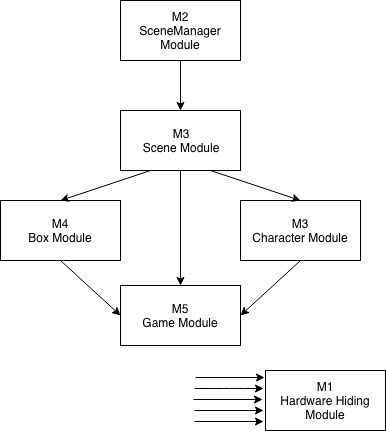
\includegraphics[width=0.7\textwidth]{UsesHierarchy.jpg}
\caption{Use hierarchy among modules}
\label{FigUH}
\end{figure}


%\section*{References}

\bibliographystyle {plainnat}
\bibliography {MG}

\end{document}